\documentclass[]{book}
\usepackage{lmodern}
\usepackage{amssymb,amsmath}
\usepackage{ifxetex,ifluatex}
\usepackage{fixltx2e} % provides \textsubscript
\ifnum 0\ifxetex 1\fi\ifluatex 1\fi=0 % if pdftex
  \usepackage[T1]{fontenc}
  \usepackage[utf8]{inputenc}
\else % if luatex or xelatex
  \ifxetex
    \usepackage{mathspec}
  \else
    \usepackage{fontspec}
  \fi
  \defaultfontfeatures{Ligatures=TeX,Scale=MatchLowercase}
\fi
% use upquote if available, for straight quotes in verbatim environments
\IfFileExists{upquote.sty}{\usepackage{upquote}}{}
% use microtype if available
\IfFileExists{microtype.sty}{%
\usepackage{microtype}
\UseMicrotypeSet[protrusion]{basicmath} % disable protrusion for tt fonts
}{}
\usepackage[margin=1in]{geometry}
\usepackage{hyperref}
\hypersetup{unicode=true,
            pdftitle={Pedologia Quantitativa feita Simples},
            pdfauthor={Alessandro Samuel-Rosa},
            pdfborder={0 0 0},
            breaklinks=true}
\urlstyle{same}  % don't use monospace font for urls
\usepackage{natbib}
\bibliographystyle{apalike}
\usepackage{color}
\usepackage{fancyvrb}
\newcommand{\VerbBar}{|}
\newcommand{\VERB}{\Verb[commandchars=\\\{\}]}
\DefineVerbatimEnvironment{Highlighting}{Verbatim}{commandchars=\\\{\}}
% Add ',fontsize=\small' for more characters per line
\usepackage{framed}
\definecolor{shadecolor}{RGB}{248,248,248}
\newenvironment{Shaded}{\begin{snugshade}}{\end{snugshade}}
\newcommand{\KeywordTok}[1]{\textcolor[rgb]{0.13,0.29,0.53}{\textbf{{#1}}}}
\newcommand{\DataTypeTok}[1]{\textcolor[rgb]{0.13,0.29,0.53}{{#1}}}
\newcommand{\DecValTok}[1]{\textcolor[rgb]{0.00,0.00,0.81}{{#1}}}
\newcommand{\BaseNTok}[1]{\textcolor[rgb]{0.00,0.00,0.81}{{#1}}}
\newcommand{\FloatTok}[1]{\textcolor[rgb]{0.00,0.00,0.81}{{#1}}}
\newcommand{\ConstantTok}[1]{\textcolor[rgb]{0.00,0.00,0.00}{{#1}}}
\newcommand{\CharTok}[1]{\textcolor[rgb]{0.31,0.60,0.02}{{#1}}}
\newcommand{\SpecialCharTok}[1]{\textcolor[rgb]{0.00,0.00,0.00}{{#1}}}
\newcommand{\StringTok}[1]{\textcolor[rgb]{0.31,0.60,0.02}{{#1}}}
\newcommand{\VerbatimStringTok}[1]{\textcolor[rgb]{0.31,0.60,0.02}{{#1}}}
\newcommand{\SpecialStringTok}[1]{\textcolor[rgb]{0.31,0.60,0.02}{{#1}}}
\newcommand{\ImportTok}[1]{{#1}}
\newcommand{\CommentTok}[1]{\textcolor[rgb]{0.56,0.35,0.01}{\textit{{#1}}}}
\newcommand{\DocumentationTok}[1]{\textcolor[rgb]{0.56,0.35,0.01}{\textbf{\textit{{#1}}}}}
\newcommand{\AnnotationTok}[1]{\textcolor[rgb]{0.56,0.35,0.01}{\textbf{\textit{{#1}}}}}
\newcommand{\CommentVarTok}[1]{\textcolor[rgb]{0.56,0.35,0.01}{\textbf{\textit{{#1}}}}}
\newcommand{\OtherTok}[1]{\textcolor[rgb]{0.56,0.35,0.01}{{#1}}}
\newcommand{\FunctionTok}[1]{\textcolor[rgb]{0.00,0.00,0.00}{{#1}}}
\newcommand{\VariableTok}[1]{\textcolor[rgb]{0.00,0.00,0.00}{{#1}}}
\newcommand{\ControlFlowTok}[1]{\textcolor[rgb]{0.13,0.29,0.53}{\textbf{{#1}}}}
\newcommand{\OperatorTok}[1]{\textcolor[rgb]{0.81,0.36,0.00}{\textbf{{#1}}}}
\newcommand{\BuiltInTok}[1]{{#1}}
\newcommand{\ExtensionTok}[1]{{#1}}
\newcommand{\PreprocessorTok}[1]{\textcolor[rgb]{0.56,0.35,0.01}{\textit{{#1}}}}
\newcommand{\AttributeTok}[1]{\textcolor[rgb]{0.77,0.63,0.00}{{#1}}}
\newcommand{\RegionMarkerTok}[1]{{#1}}
\newcommand{\InformationTok}[1]{\textcolor[rgb]{0.56,0.35,0.01}{\textbf{\textit{{#1}}}}}
\newcommand{\WarningTok}[1]{\textcolor[rgb]{0.56,0.35,0.01}{\textbf{\textit{{#1}}}}}
\newcommand{\AlertTok}[1]{\textcolor[rgb]{0.94,0.16,0.16}{{#1}}}
\newcommand{\ErrorTok}[1]{\textcolor[rgb]{0.64,0.00,0.00}{\textbf{{#1}}}}
\newcommand{\NormalTok}[1]{{#1}}
\usepackage{longtable,booktabs}
\usepackage{graphicx,grffile}
\makeatletter
\def\maxwidth{\ifdim\Gin@nat@width>\linewidth\linewidth\else\Gin@nat@width\fi}
\def\maxheight{\ifdim\Gin@nat@height>\textheight\textheight\else\Gin@nat@height\fi}
\makeatother
% Scale images if necessary, so that they will not overflow the page
% margins by default, and it is still possible to overwrite the defaults
% using explicit options in \includegraphics[width, height, ...]{}
\setkeys{Gin}{width=\maxwidth,height=\maxheight,keepaspectratio}
\IfFileExists{parskip.sty}{%
\usepackage{parskip}
}{% else
\setlength{\parindent}{0pt}
\setlength{\parskip}{6pt plus 2pt minus 1pt}
}
\setlength{\emergencystretch}{3em}  % prevent overfull lines
\providecommand{\tightlist}{%
  \setlength{\itemsep}{0pt}\setlength{\parskip}{0pt}}
\setcounter{secnumdepth}{5}
% Redefines (sub)paragraphs to behave more like sections
\ifx\paragraph\undefined\else
\let\oldparagraph\paragraph
\renewcommand{\paragraph}[1]{\oldparagraph{#1}\mbox{}}
\fi
\ifx\subparagraph\undefined\else
\let\oldsubparagraph\subparagraph
\renewcommand{\subparagraph}[1]{\oldsubparagraph{#1}\mbox{}}
\fi

%%% Use protect on footnotes to avoid problems with footnotes in titles
\let\rmarkdownfootnote\footnote%
\def\footnote{\protect\rmarkdownfootnote}

%%% Change title format to be more compact
\usepackage{titling}

% Create subtitle command for use in maketitle
\newcommand{\subtitle}[1]{
  \posttitle{
    \begin{center}\large#1\end{center}
    }
}

\setlength{\droptitle}{-2em}
  \title{Pedologia Quantitativa feita Simples}
  \pretitle{\vspace{\droptitle}\centering\huge}
  \posttitle{\par}
  \author{Alessandro Samuel-Rosa}
  \preauthor{\centering\large\emph}
  \postauthor{\par}
  \predate{\centering\large\emph}
  \postdate{\par}
  \date{2016-09-21}

\usepackage{booktabs}

\begin{document}
\maketitle

{
\setcounter{tocdepth}{1}
\tableofcontents
}
\chapter{Introdução}\label{intro}

\chapter*{PARTE \_\_ -- INFRAESTRUTURA}\label{parte-__-infraestrutura}
\addcontentsline{toc}{chapter}{PARTE \_\_ -- INFRAESTRUTURA}

\chapter{SOFTWARE}\label{software}

\section{R/RStudio}\label{rrstudio}

O R é uma linguagem de programação e um ambiente de análises
estatísticas e gráficas. Sua origem data de 1995, quando dois
pesquisadores (Robert Gentleman e Ross Ihaka) iniciaram o projeto de seu
desenvolvimento no Departamento de Estatística da Universidade de
Auckland na Nova Zelândia. O nome deriva, exatamente, das iniciais dos
dois pesquisadores: R.

Atualmente o R está disponível como um Software Livre sob os termos da
Licença Pública Geral do GNU da Fundação do Software Livre na forma de
código fonte. Isso quer dizer que o R está disponível gratuitamente para
qualquer interessado em utilizá-lo, seja para atividades com ou sem fins
lucrativos. Além disso, essa licença permite que o usuário faça
alterações conforme desejado. Tanto o aplicativo como as alterações
podem ser reproduzidas e distribuídas, desde que sempre mantidos os
direitos dos autores.

Enfim, a grande vantagem do R em relação à maioria dos \emph{softwares}
de análise estatística disponíveis no mercado é exatamente a sua
gratuidade. Mas essa gratuidade não é, como em alguns casos, sinônimo de
baixa qualidade. Pelo contrário, o R possui uma série de funcionalidades
muitas vezes ainda não implementadas em softwares comercializados. Todo
tipo de análise pode ser realizada utilizando o R: basta que já exista
um pacote que a implemente ou que o usuário desenvolva o código. Além
disso, o R permite que as rotinas de análise sejam registradas e, quando
necessário, verificadas ou disponibilizadas para verificação por outros
pesquisadores. Trata-se de uma funcionalidade que possibilita
verdadeiramente a observação de alguns dos princípios do método
científico.

A gratuidade do R por si só já deveria ser suficiente para convencer
nossos pesquisadores, que dispõe de recursos escassos para manter as
licenças dos softwares comerciais, a usar o R. Mas não é só isso! O R é
hoje o que a maioria dos estatísticos e matemáticos ao redor do mundo
utiliza para analisar seus dados. São esses estatísticos e matemáticos
que estão ajudando a desenvolver o R mais e mais. Além disso, são esses
profissionais que disponibilizam parte de seu tempo para elaborar a
miríade de tutoriais e materiais de apoio disponíveis atualmente. Nenhum
software comercial possui, hoje, seja em meio digital como em meio
impresso, um volume de material de apoio maior do que o R. Soma-se ainda
o fato de que o R permite a confecção de gráficos de qualidade igual ou
até superior a qualquer pacote comercial disponível hoje no mercado.
Além disso, o R roda em qualquer sistema operacional. Será que é preciso
dizer mais alguma coisa?

\subsection{Conhecendo melhor o R}\label{conhecendo-melhor-o-r}

A melhor maneira de conhecer melhor o R é, sem dúvida, instalando-o em
seu computador. Para isso precisamos, primeiro, visitar a página do
projeto na Internet:

\begin{verbatim}
## PhantomJS not found. You can install it with webshot::install_phantomjs(). If it is installed, please make sure the phantomjs executable can be found via the PATH variable.
\end{verbatim}

Uma grande quantidade de informação, muito além do que se busca incluir
neste livro, pode ser encontrada no sítio do projeto. Ali estão
disponíveis diversos manuais de uso
(\texttt{Documentation\ \textgreater{}\ Munuals}), bem como livros
(\texttt{Documentation\ \textgreater{}\ Books}) e artigos publicados na
revista do projeto
(\texttt{Documentation\ \textgreater{}\ The\ R\ Journal}). Ainda há uma
página com respostas às perguntas mais frequentes
(\texttt{Documentation\ \textgreater{}\ FAQs}) e uma página inteira
explicando sobre como é possível conseguir ajuda do próprio R antes de
recorrer a terceiros
(\texttt{Help\ With\ R\ \textgreater{}\ Getting\ Help}) -- como a
documentação do R é extensa e a maioria dos colaboradores do projeto não
são pagos pela colaboração, recomendo que você sempre procure, primeiro,
resolver qualquer dúvida sozinho.

O procedimento de instalação do R depende do sistema operacional
(\href{https://en.wikipedia.org/wiki/Operating_system}{OS}, do inglês
\emph{operating system}) de seu computador:

\begin{itemize}
\tightlist
\item
  Linux: \url{https://cloud.r-project.org/bin/linux/}
\item
  (Mac) OS X: \url{https://cloud.r-project.org/bin/macosx/}
\item
  Windows: \url{https://cloud.r-project.org/bin/windows/base/}
\end{itemize}

A página referente à cada OS possui as instruções necessárias para
descarregar e instalar o R em seu computador. Em geral, o processo de
instalação é exatamente igual àquele de outros \emph{softwares} que você
usa em seu dia-a-dia.

Depois de instalar o R, agora é a hora de escolher uma interface gráfica
do usuário
(\href{https://en.wikipedia.org/wiki/Graphical_user_interface}{GUI}, do
inglês \emph{graphical user interface}) que facilite nossa interação com
o R. Isso porque o R possui apenas uma interface de linha de comando
(\href{https://en.wikipedia.org/wiki/Command-line_interface}{CLI}, do
inglês \emph{command-line interface}), ou seja, a única forma de
interação com o R se dá via emissão de comandos sob a forma de
sucessivas linhas de texto, as chamadas linhas de comando. Dentre as
diversas opções gratuitamente disponíveis, as mais atrativas são aquelas
que incluem ferramentas adicionais de apoio à programação em R e
facilitem a análise, visualização e gerenciamento dos dados. Tais
ferramentas constituem os chamados ambientes de desenvolvimento
integrado
(\href{https://en.wikipedia.org/wiki/Integrated_development_environment}{IDE},
do inglês \emph{integrated development environment}). Atualmente, a GUI
e IDE mais popular é o RStudio, cujo instalador pode ser descarregado de
\url{https://www.rstudio.com/products/rstudio/download/}.

Assim como para o R, o procedimento de instalação do RStudio depende do
OS do seu computador. Depois de instalado, inicie o RStudio em seu
computador. Ele deve se parecer mais ou menos como na figura a seguir:

\begin{figure}[htbp]
\centering
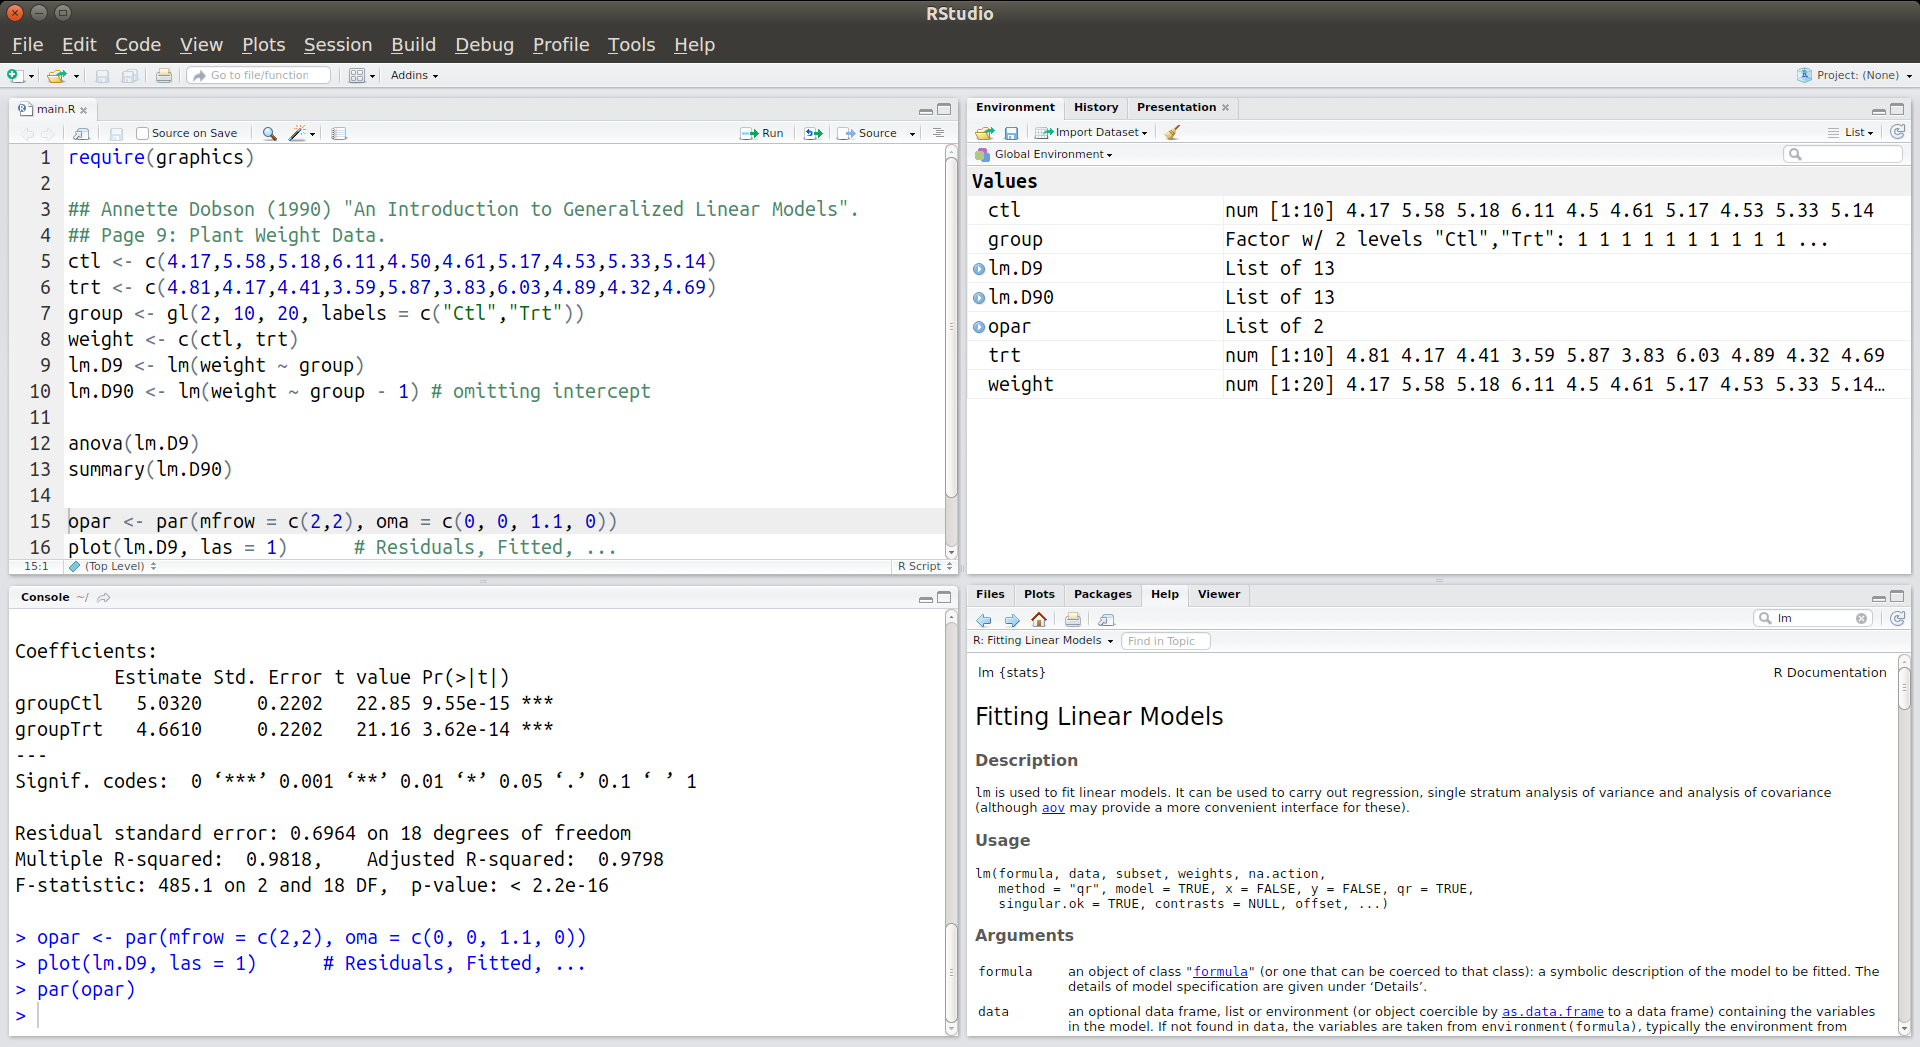
\includegraphics{images/rstudio-snapshot.png}
\caption{RStudio -- interface gráfica do usuário e ambiente de
desenvolvimento integrado para R (em sua versão para Linux). Uma extensa
lista de alternativas está disponível na
\href{https://en.wikipedia.org/wiki/R_(programming_language)\#Interfaces}{Wikipedia}.}
\end{figure}

Você deve ter notado que o RStudio é composto por quatro grandes painéis
retangulares, cada um contendo conteúdo específico. Grosso modo, o
painel superior direito mostra informações diversas sobre a atual sessão
de trabalho, sendo geralmente pouco utilizado. Já o painel inferior
direito serve à visualização de gráficos e páginas de ajuda do R, o que
o faz ser bastante utilizado. O painel superior esquerdo é aquele
utilizado para a programação em R, ou seja, aquele onde o código fonte
utilizado para a análise dos dados é editado. Esse painel é aquele onde
creio que ocupamos a maior parte do tempo. Por fim, o painel inferior
esquerdo corresponde à interface de linha de comando, CLI, do R. É ali
que o código fonte editado no painel superior esquerdo deve ser emitido
para que a mágica aconteça.

\subsection{Primeiros passos}\label{primeiros-passos}

Façamos algumas operações matemáticas para nos familiarizarmos com o R.
Você pode copiar e colar as linhas de código abaixo no CLI do R, que de
agora em diante chamaremos \textbf{\emph{console}}.

\begin{Shaded}
\begin{Highlighting}[]
\CommentTok{# As quatro operações matemáticas básicas:}
\DecValTok{2} \NormalTok{+}\StringTok{ }\DecValTok{3} \CommentTok{# soma}
\end{Highlighting}
\end{Shaded}

\begin{verbatim}
## [1] 5
\end{verbatim}

\begin{Shaded}
\begin{Highlighting}[]
\DecValTok{5}\NormalTok{*}\StringTok{ }\DecValTok{5} \CommentTok{# multiplicação}
\end{Highlighting}
\end{Shaded}

\begin{verbatim}
## [1] 25
\end{verbatim}

\begin{Shaded}
\begin{Highlighting}[]
\DecValTok{25}\NormalTok{/}\DecValTok{5} \CommentTok{# divisão }
\end{Highlighting}
\end{Shaded}

\begin{verbatim}
## [1] 5
\end{verbatim}

\begin{Shaded}
\begin{Highlighting}[]
\DecValTok{5} \NormalTok{-}\DecValTok{3} \CommentTok{# subtração}
\end{Highlighting}
\end{Shaded}

\begin{verbatim}
## [1] 2
\end{verbatim}

\begin{Shaded}
\begin{Highlighting}[]
\CommentTok{# Três operações matemáticas úteis:}
\DecValTok{2}\NormalTok{^}\DecValTok{2}      \CommentTok{# Potenciação (ou exponenciação)}
\end{Highlighting}
\end{Shaded}

\begin{verbatim}
## [1] 4
\end{verbatim}

\begin{Shaded}
\begin{Highlighting}[]
\KeywordTok{log}\NormalTok{(}\DecValTok{4}\NormalTok{)   }\CommentTok{# Função logarítmica}
\end{Highlighting}
\end{Shaded}

\begin{verbatim}
## [1] 1.386294
\end{verbatim}

\begin{Shaded}
\begin{Highlighting}[]
\KeywordTok{sqrt}\NormalTok{(}\DecValTok{25}\NormalTok{) }\CommentTok{# Raiz quadrada}
\end{Highlighting}
\end{Shaded}

\begin{verbatim}
## [1] 5
\end{verbatim}

Você deve ter notado que que os símbolos utilizados (\texttt{+},
\texttt{*}, \texttt{/} e \texttt{-}) são os mesmos encontrados em
qualquer calculadora científica. São também os mesmos utilizados nas
operações matemáticas de qualquer planilha eletrônica de edição de
dados. Isso significa que podemos deduzir muitas coisas sobre o
funcionamento do R a partir do que conhecemos de outros \emph{softwares}
dedicados à análise e manipulação de dados. Você também deve ter
observado que o espaçamento entre número e operador matemático não tem
qualquer importância do ponto de vista da operação matemática. Contudo,
do ponto de vista estético -- para facilidade de leitura do código fonte
--, costuma-se usar a formatação \texttt{2\ +\ 3} ao invés de
\texttt{2+3}.

Outro detalhe importante nas linhas de código acima é o uso do símbolo
\texttt{\#} para a inclusão de comentários. Os comentários podem ser
incluídos tanto em uma linha própria como após (nunca antes) um comando.
A inclusão de comentários no código fonte é fundamental para
documentarmos a atividade que estamos realizando a fim de que outros (e
nós mesmos, algumas semanas ou meses mais tarde) possamos entender o
propósito daquelas linhas de código.

Finalmente, você deve ter notado que as duas últimas operações
matemáticas foram feitas usando uma declaração nominal e dois
parênteses, ou seja, \texttt{log()} para a função logarítmica e
\texttt{sqrt()} para a raiz quadrada. Na verdade, \texttt{log()} e
\texttt{sqrt()} são \textbf{\emph{funções}} do R, assim como
\texttt{sum()} (soma), \texttt{diff()} (diferença), entre outras. Uma
função arbitrária chamada \texttt{fun()} sempre é usada da seguinte
maneira: \texttt{fun(x)}, onde \texttt{x} é um argumento qualquer (um
número, por exemplo) tomado pela função. Por exemplo, uma função
bastante conhecida entre nós é aquela da Lei Básica da Ciência do Solo,

\[solo = f(cl, o, r, p, t, \ldots)\]

onde \(cl\) representa o clima, \(o\) representa os organismos vivos,
incluindo nós seres humanos, \(r\) significa relevo, \(p\) é o material
parental, \(t\) representa o tempo e \(\ldots\) são fatores não
conhecidos ou de limitada relevância. Em R, essa função seria escrita
extamente da seguinte forma: \texttt{solo(cl,\ o,\ r,\ p,\ t,\ ...)}.
Vejamos mais um exemplo, agora de uma função que aceita vários
argumentos:

\begin{Shaded}
\begin{Highlighting}[]
\CommentTok{# No RStudio, ponha o cursor sobre o nome da função e pressione 'F1' para ver a }
\CommentTok{# sua página de ajuda. Lá você verá o nome dos argumentos aceitos pela função }
\CommentTok{# 'plot()' seguido de uma breve descrição.}
\KeywordTok{plot}\NormalTok{(}\DataTypeTok{x =} \DecValTok{25}\NormalTok{, }\DataTypeTok{y =} \DecValTok{25}\NormalTok{, }\DataTypeTok{col =} \StringTok{"red"}\NormalTok{, }\DataTypeTok{main =} \StringTok{"Um ponto vermelho"}\NormalTok{, }\DataTypeTok{xlab =} \StringTok{"x"}\NormalTok{, }\DataTypeTok{ylab =} \StringTok{"y"}\NormalTok{)}
\end{Highlighting}
\end{Shaded}

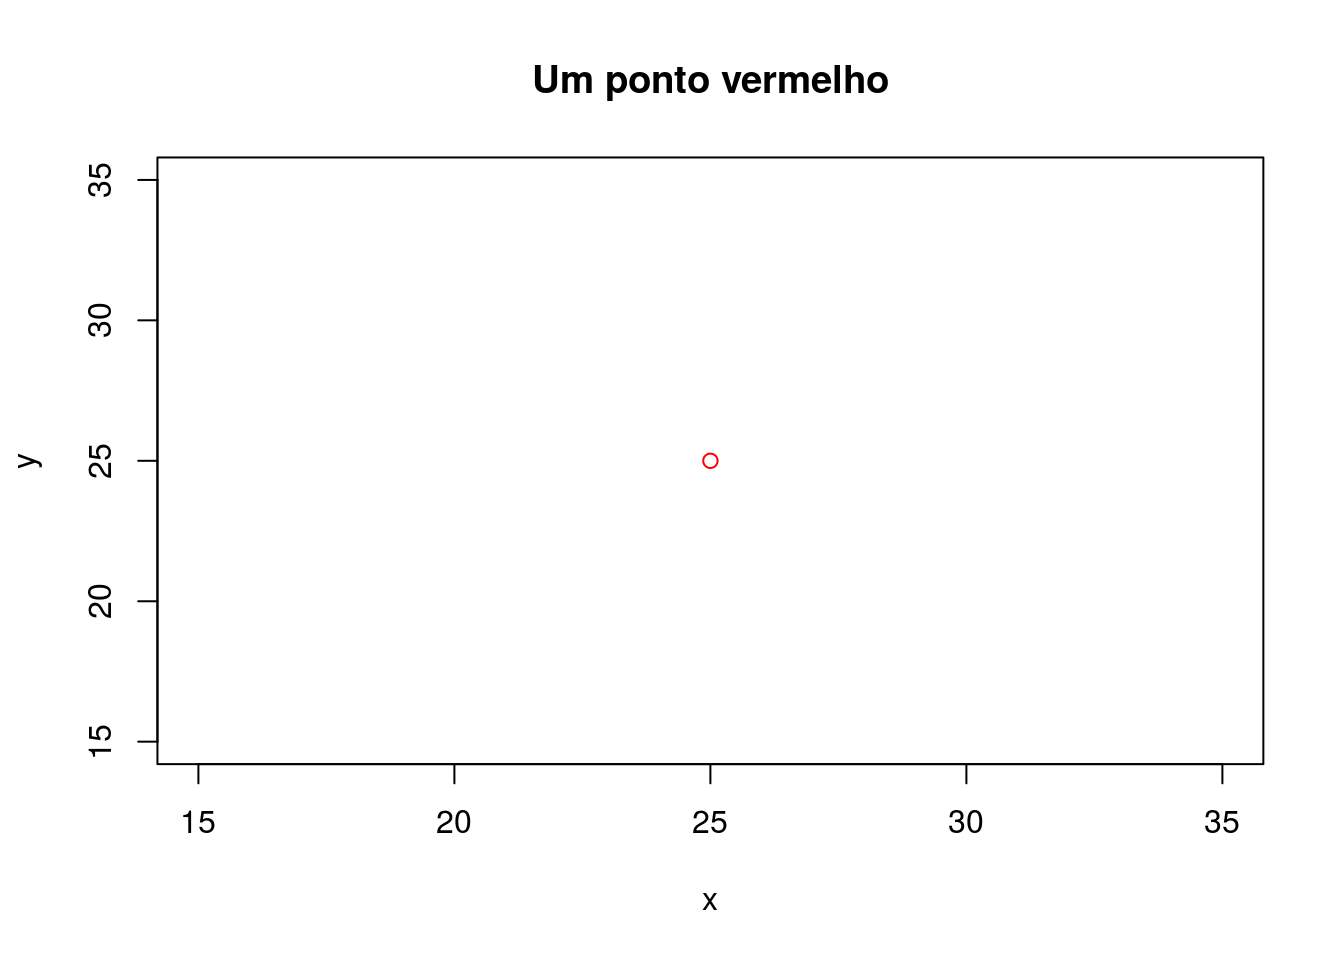
\includegraphics{pedologia-quantitativa_files/figure-latex/unnamed-chunk-2-1.pdf}

\subsection{Conceitos básicos}\label{conceitos-basicos}

Passada a primeira impressão, agora precisamos nos familiarizar com
alguns conceitos básicos para que possamos entender o R e utilizá-lo com
êxito. Conforme destacado acima, o R não é um simples \emph{software}
para análises estatísticas, mas sim um ambiente de programação. E, para
isso, precisamos de uma linguagem de programação, ou seja, a linguagem
de programação R. Como sabemos, uma linguagem é um sistema de signos
(símbolos ou palavras) convencionados que serve para a comunicação de
conceitos, ideias, significados, pensamentos -- veja mais sobre
linguagem na
\href{\%22https://pt.wikipedia.org/wiki/Linguagem\%22}{Wikipedia}.
Assim, uma linguagem de programação será, também, um sistema de signos
convencionados, mas que serve para a nossa comunicação com um
computador, especificamente, para dar instruções a um computador. Sendo
uma linguagem, haverá regras sintáticas e semânticas (uma gramática), as
quais devem ser estritamente respeitadas para que haja, efetivamente,
comunicação entre nós e o computador -- veja mais sobre linguagem de
programação na
\href{https://pt.wikipedia.org/wiki/Linguagem_de_programa\%C3\%A7\%C3\%A3o}{Wikipedia}

A gramática de uma linguagem de programação possui dois elementos
principais: as palavras reservadas e as palavras-chave. As
\textbf{\emph{palavras reservadas}} constituem signos com significado
especial para a linguagem de programação, definidas internamente no
código fonte, e que não podem ser utilizadas pelo usuário para fins
outros que não aqueles especificados internamente pelo \emph{software}
(por exemplo, para identificar objetos e funções -- veremos esses
conceitos a seguir). Algumas das palavras reservadas do R são
\texttt{if}, \texttt{else}, \texttt{while}, \texttt{TRUE} e
\texttt{FALSE}. No editor de código fonte do RStudio as palavras
reservadas aparecem sempre destacadas em azul -- busque pelo termo
\emph{reserved} no painel de ajuda do RStudio para conhecer as palavras
reservadas do R.

As \textbf{\emph{palavras-chave}} são aquelas utilizadas para definir
funções (e objetos, como veremos a seguir). As palavras-chave que
definem funções são aquelas que acionam operações matemáticas e lógicas
que possibilitam, por exemplo, a realização de uma determinada análise
estatística de um determinado conjunto de dados -- na verdade, tudo o
que ``acontece'' no R acontece pela ação de uma função. As
palavras-chave que definem funções podem já estar definidas na própria
linguagem de programação -- como \texttt{log}, \texttt{sqrt} e
\texttt{plot} nos exemplos acima -- ou ser criadas pelo usuário. Isso
significa que o usuário pode criar suas próprias funções conforme sua
necessidade. Vejamos um exemplo:

\begin{Shaded}
\begin{Highlighting}[]
\CommentTok{# A palavra-chave 'soma' é usada para definir uma função que computa}
\CommentTok{# e retorna como resultado `res` a soma de dois valores numéricos.}
\CommentTok{# A estrutura da função aparece, sempre, entre '\{' e '\}'.}
\NormalTok{soma <-}\StringTok{ }
\StringTok{  }\NormalTok{function (x, y) \{ }
    \NormalTok{res <-}\StringTok{ }\NormalTok{x +}\StringTok{ }\NormalTok{y}
    \KeywordTok{return} \NormalTok{(res)}
    \NormalTok{\}}
\KeywordTok{soma}\NormalTok{(}\DataTypeTok{x =} \DecValTok{2}\NormalTok{, }\DataTypeTok{y =} \DecValTok{2}\NormalTok{)}
\end{Highlighting}
\end{Shaded}

\begin{verbatim}
## [1] 4
\end{verbatim}

Você deve ter notado que duas palavras reservadas foram usadas na
construção da função \texttt{soma()}. São elas: \texttt{function} e
\texttt{return}. Além disso, uma segunda palavra-chave foi usada:
\texttt{res}. Essa palavra-chave foi usada para definir um objeto que
armazena o resultado da operação matemática realizada pela função
\texttt{soma()}. Assim, na verdade, a função \texttt{soma()} não retorna
o resultado da operação matemática, mas sim um objeto que armazena o seu
resultado. Grosso modo, um \textbf{\emph{objeto}} nada mais é do que uma
estrutura de dados -- como diria John Chambers, tudo o que ``existe'' no
R é um objeto. Essas estruturas de dados são vetores, matrizes, listas e
outras estruturas de dados inseridas ou criadas pelo próprio usuário ou
produzidas como resultado dos diversos procedimentos analíticos. Vejamos
alguns exemplos para nos familiarizamos como esse conceito.

Imagine dois vetores de dados \(x = [1, 2, 3, 4, 5]\) e
\(y = [2, 4, 3, 5, 7]\). Esses vetores são inseridos no R e nomeados,
respectivamente, como \texttt{x} e \texttt{y}. Então, \texttt{x} e
\texttt{y} passam a ser palavras-chave que identificam dois objetos, ou
seja, uma estrutura de dados, nesse caso, vetores. Ao emitirmos uma
chamada dos objetos \texttt{x} e \texttt{y}, o R retorna os respectivos
valores neles armazenados:

\begin{Shaded}
\begin{Highlighting}[]
\CommentTok{# Definindo dois objetos vetoriais}
\CommentTok{# Note que quando criamos uma sequência ordenada de valores podemos }
\CommentTok{# simplesmente usar o símbolo ':' entre o menor e o maior valor da }
\CommentTok{# sequência ao invés de declarar todos os seus valores.}
\NormalTok{x <-}\StringTok{ }\DecValTok{1}\NormalTok{:}\DecValTok{5}
\NormalTok{y <-}\StringTok{ }\KeywordTok{c}\NormalTok{(}\DecValTok{2}\NormalTok{, }\DecValTok{4}\NormalTok{, }\DecValTok{3}\NormalTok{, }\DecValTok{5}\NormalTok{, }\DecValTok{7}\NormalTok{)}
\NormalTok{x}
\end{Highlighting}
\end{Shaded}

\begin{verbatim}
## [1] 1 2 3 4 5
\end{verbatim}

\begin{Shaded}
\begin{Highlighting}[]
\NormalTok{y}
\end{Highlighting}
\end{Shaded}

\begin{verbatim}
## [1] 2 4 3 5 7
\end{verbatim}

Suponha agora que estejamos interessados na construção de um modelo de
regressão linear, para a qual usamos a função \texttt{lm()}, do vetor
\(y\) em função do vetor \(x\):

\begin{Shaded}
\begin{Highlighting}[]
\CommentTok{# Calibração de um modelo de regressão linear}
\CommentTok{# Note que é possível usar simbolos como '.' e '_' na construção de }
\CommentTok{# uma palavra-chave identificadora de objeto (ou função).}
\NormalTok{meu.modelo_linear <-}\StringTok{ }\KeywordTok{lm}\NormalTok{(y ~}\StringTok{ }\NormalTok{x)}
\NormalTok{meu.modelo_linear}
\end{Highlighting}
\end{Shaded}

\begin{verbatim}
## 
## Call:
## lm(formula = y ~ x)
## 
## Coefficients:
## (Intercept)            x  
##         0.9          1.1
\end{verbatim}

Nesse exemplo, o objeto identificado pela palavra-chave
\texttt{meu.modelo\_linear} constitui uma estrutura de dados que contém
todas as especificações do modelo de regressão linear de \(y\) em função
de \(x\). Ao emitirmos uma chamada ao objeto \texttt{meu.modelo\_linear}
o R retorna os coeficientes do modelo de regressão linear calibrado. Se
você quiser conhecer mais sobre a estrutura do objeto
\texttt{meu.modelo\_linear}, use o seguinte comando:
\texttt{str(meu.modelo\_linear)}. Como sugestão, use também os comandos
\texttt{anova(meu.modelo\_linear)}, \texttt{summary(meu.modelo\_linear)}
e \texttt{plot(meu.modelo\_linear)}.

Você deve ter notado nos exemplos acima que a atribuição de uma
palavra-chave à um objeto ou à uma função está sempre atrelada ao uso do
símbolo \texttt{\textless{}-}. Por exemplo,
\texttt{x\ \textless{}-\ 1:5} atribui a palavra-chave \texttt{x} ao
objeto de estrutura vetorial contendo valores numéricos de 1 até 5. A
atribuição também pode ser feita usando o símbolo \texttt{=}. Contudo,
como \texttt{=} também pode ser usado em contextos outros que não a
atribuição de palavras-chave, o uso de \texttt{\textless{}-} costuma ser
preferido.

Nesse ponto você já deve ter percebido que, para usar o R, será preciso
aprender uma nova linguagem, um novo sistema de signos. Alguma coisa
poderá ser deduzida a partir daquilo que já sabemos em função do uso de
outros \emph{softwares} de análise e processamento de dados. Contudo,
como qualquer linguagem de programação, o R possui suas especificidades,
boa parte das quais é preciso conhecer para termos sucesso em seu uso.
Além disso, algum conhecimento da língua inglesa será necessário, haja
vista que as palavras reservadas e palavras-chave são derivadas de
palavras da língua inglesa, e praticamente toda a (extensa) documentação
está disponível apenas em inglês. A partir de agora estamos,
oficialmente, nos domínios do Vale da Morte:

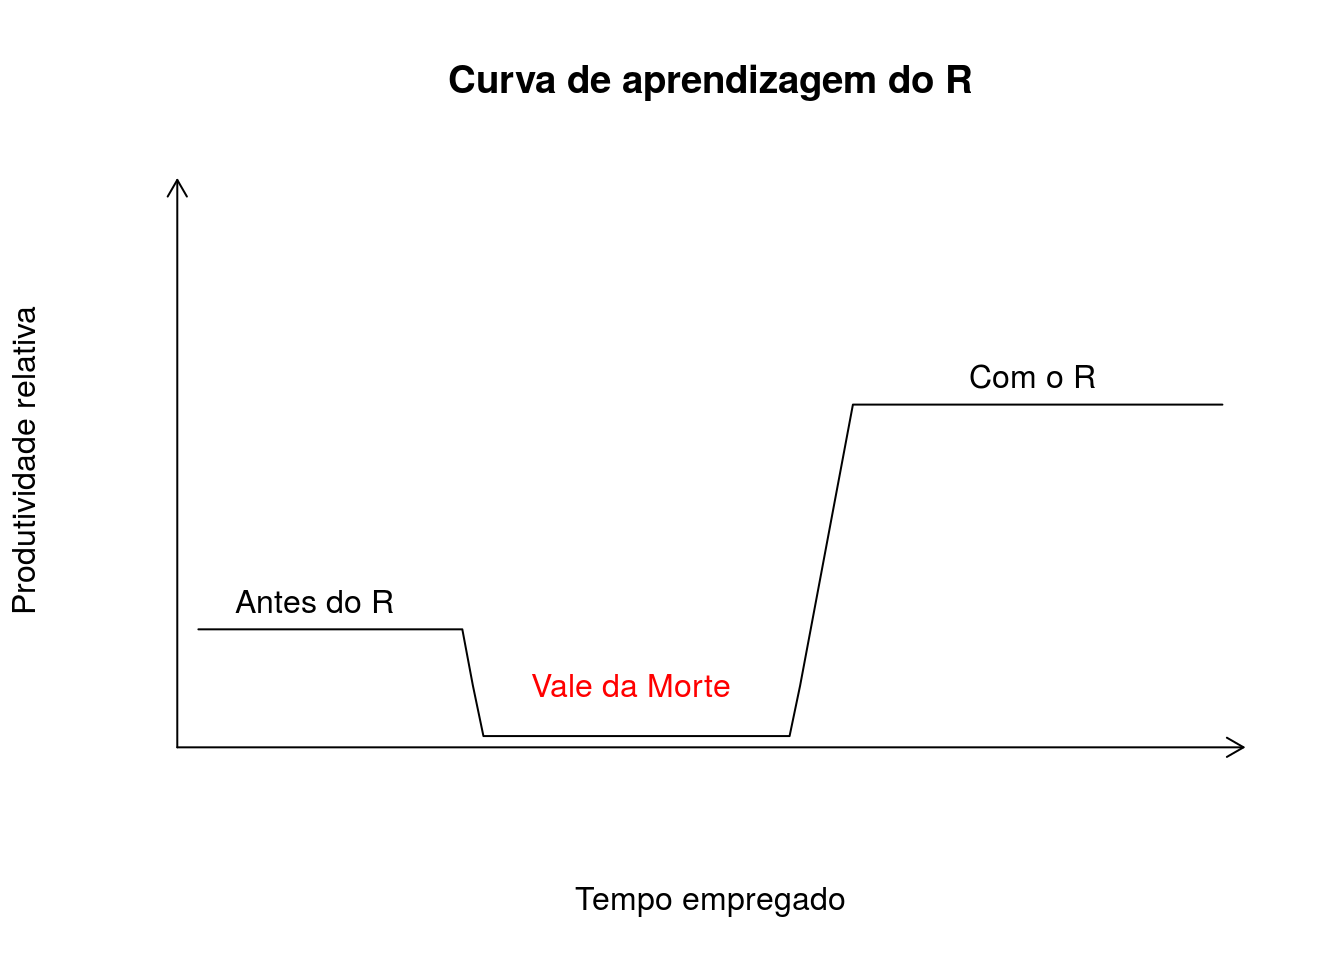
\includegraphics{pedologia-quantitativa_files/figure-latex/unnamed-chunk-6-1.pdf}

\subsection{Os pacotes}\label{os-pacotes}

Um pacote constitui uma coleção de arquivos e diretórios que contém as
regras sintáticas e semânticas que definem determinadas operações
matemáticas e lógicas. Na instalação padrão do R um conjunto de pacotes
já está incluído. Esses pacotes permitem que uma determinada gama de
análises estatísticas sejam realizadas. Cada pacote possui um nome
específico e ficam armazenados no diretório de instalação do R. São
exemplos os pacotes `base' e `stats'.

Mas as capacidades do R podem ser estendidas através da instalação de
novos pacotes. Esses pacotes irão conter as regras sintáticas e
semânticas que também definem operações matemáticas e lógicas permitindo
a realização de novos métodos de análise estatística e gráfica. São
exemplos os pacotes `chemometrics' e `agricolae'.

Para instalar um novo pacote deve-se clicar na barra de menus localizada
no topo da interface em Pacotes \textgreater{} Instalar
pacote(s)\ldots{} e então seleciona-se o espelho (CRAN mirror) mais
próximo. Na lista que aparece são selecionados os pacotes desejados.
Clique em OK.

Depois de instalado o pacote é preciso carregá-lo. Para isso dirija-se
novamente até a barra de menus localizada no topo da interface e clique
em Pacotes \textgreater{} Carregar pacote e selecione na lista o pacote
desejado. Toda vez que o R é iniciado apenas os pacotes básicos (já
presentes na instalação padrão) são carregados automaticamente. Os
pacotes instalados posteriormente através do procedimento descrito acima
devem ser carregados manualmente.

\begin{Shaded}
\begin{Highlighting}[]
\KeywordTok{install.packages}\NormalTok{(}
  \KeywordTok{c}\NormalTok{(}\StringTok{"sp"}\NormalTok{, }\StringTok{"raster"}\NormalTok{, }\StringTok{"rgdal"}\NormalTok{, }\StringTok{"pedometrics"}\NormalTok{, }\StringTok{"randomForest"}\NormalTok{, }\StringTok{"rsaga"}\NormalTok{), }\DataTypeTok{dependencies =} \OtherTok{TRUE}\NormalTok{)}
\end{Highlighting}
\end{Shaded}

\subsection{Comandos e símbolos}\label{comandos-e-simbolos}

Conforme mostrado nos quadros acima, todas as funcionalidades do R são
acionadas através do uso de comandos de texto e símbolos (matemáticos ou
não). Esses comandos e símbolos já estão definidos na linguagem do R e,
por isso, quando utilizados, devem ser inseridos de maneira correta para
que sejam efetivamente reconhecidos. Assim, é importante ter cuidado
porque o R é sensível ao uso de letras maiúsculas e minúsculas, bem como
a acentuação e uso de cedilha.

Basta pressionar a tecla `enter' para acionar um comando. Caso o comando
não esteja sintaticamente completo o R mostra o símbolo `+'. Nesse caso
é preciso verificar o que está faltando no comando inserido. Note que
esse aviso não constitui uma mensagem de erro, ou seja, não há
necessidade de reescrever o comando, mas apenas completar o que falta.
Em alguns casos, se a linha de comando for muito extensa é possível
mudar para a linha seguinte e nela continuar o comando sem que isso
implique em erros.

Um comando de grande utilidade é o `help(nome\_do\_comando)' ou apenas
`?nome\_do\_comando'. Esses comandos permitem acionar a ajuda do R sobre
os diversos comandos. Contudo, seu uso exige conexão com a Internet, uma
vez que a página de ajuda do R encontra-se online. Para acessos offline
clique em Ajuda na barra de ferramentas do R.

Para auxiliar no uso dos comandos e conhecer as suas funções existem
alguns cartões de referência. Clique nos nomes dos respectivos autores
dos cartões de referência abaixo para acessá-los.

\begin{itemize}
\tightlist
\item
  \href{http://cran.r-project.org/doc/contrib/Short-refcard.pdf}{Tom
  Short}
\item
  \href{http://www.psych.upenn.edu/~baron/refcard.pdf}{Jonathan Baron}
\item
  \href{http://cran.r-project.org/doc/contrib/YanchangZhao-refcard-data-mining.pdf}{Yanchang
  Zhao}
\item
  \href{http://cran.r-project.org/doc/contrib/Ricci-refcard-regression.pdf}{Vito
  Ricci}
\end{itemize}

\section{QGIS}\label{qgis}

\url{http://www.qgis.org/}

\section{SAGA GIS}\label{saga-gis}

\url{http://www.saga-gis.org/}

\section{GRASS GIS}\label{grass-gis}

\url{https://grass.osgeo.org/}

\section{GDAL}\label{gdal}

\url{http://www.gdal.org/}

\chapter{GESTÃO DE DADOS}\label{gestao-de-dados}

Um importante passo consiste na criação do nosso diretório de trabalho.
Para isso, acesse seu gerenciador de diretórios e crie a seguinte
estrutura de diretórios em seu local favorito de trabalho:

\begin{verbatim}
projeto
|- code/       # qualquer código de programação
|  |- R/       # código de programação em R
|
|- data
|  |- grid/    # dados matriciais
|  |- R/       # dados no formato *.rda
|  |- vector/  # dados vetoriais
|
|- doc/        # arquivos usados para redigir o relatório
|  |- fig/     # figuras usadas no relatório
\end{verbatim}

Note que, dentro do nosso diretório de trabalho principal
(\texttt{projeto}) existem três subdiretórios: \texttt{code},
\texttt{data} e \texttt{doc}. O primeiro deles, \texttt{code}, serve
para armazernamos os arquivos contendo código de programação em qualquer
linguagem. Para cada linguagem criamos um subsubdiretório específico.
Nesse exemplo, como usaremos apenas o R, criaremos apenas um
subsubdiretório chamado R. Ali dentro serão armazenados os
\emph{scripts} com código de programação do escritos em R.

O segundo subdiretório será utilizado para armazenarmos os dados usados
no projeto. Nesse exemplo, são três os tipos de dados que utilizaremos,
cada um armazenado em um subsubdiretório específico. No subsubdiretório
\texttt{grid} ficarão armazenados os dados matriciais, ou seja, os dados
das covariáveis e os resultados das predições espaciais. Já no
subsubdiretório \texttt{vector} ficarão armazenados os dados vetoriais,
ou seja, aqueles cuja forma de representação espacial pode ser a de
pontos, linhas e polígonos. Isso inclui os dados de solo e dos limites
da área de estudo. Por fim, o subsubdiretório R será usado para
armazenar dados diversos produzidos durante o processamento no R, os
quais serão salvos usando o formato \texttt{rda}.

O terceito e último subdiretório de nosso diretório de trabalho
\texttt{projeto}, aqui denominado \texttt{doc}, será usado para
armazenar os arquivos usados para redigir os documentos resultantes do
projeto.

No RStudio, acesse

\begin{verbatim}
Arquivo > Novo projeto > Diretório existente
\end{verbatim}

e navegue até o diretório recém criado \texttt{projeto}. Clique em
\texttt{Criar\ projeto}. Toda a estrutura de diretórios criada
recentemente aparecerá no painel direito inferior do RStudio. Agora crie
um novo arquivo do R e salve-o no diretório
\texttt{bigdata\ \textgreater{}\ code\ \textgreater{}\ R}. Será nesse
arquivo que você organizará o código em R usado para o processamento dos
dados. A criação de um projeto no RStudio facilita a organização dos
dados. Sempre que uma rotina de análises for desenvolvida no R é preciso
definir o diretório de trabalho. O diretório de trabalho constitui a
pasta em que estão localizados os arquivos contendo os dados a serem
analisados. Além disso, é no diretório de trabalho que o R salva o
histórico de trabalho contendo todas as operações realizadas.

Inicie o QGIS e acesse

\begin{verbatim}
Projeto > Novo > Salvar como
\end{verbatim}

e navegue até o diretório \texttt{projeto}. Nomeie o projeto como
\texttt{projeto}. Assim como para o RStudio, a criação de um projeto no
QGIS facilita a organização dos dados.

\chapter{Métodos}\label{metodos}

We describe our methods in this chapter.

\chapter{Amostragem}\label{amostragem}

\section{Tipos de amostragem}\label{tipos-de-amostragem}

A amostragem é um dos maiores contribuintes para os custos da modelagem
espacial do solo, seja pelo método chamado ``tradicional'' ou usando
modelos estatísticos. Assim, o adequado planejamento amostral é
essencial para reduzir a necessidade de recursos (financeiros,
psicológicos, humanos, entre outros) e maximizar o número de observações
possíveis, sejam elas tradagens, amostras superficiais, ou descrições de
perfis completos.

A \emph{situação ideal} é aquela em que os recursos disponíveis não
impõe quaisquer limitações à amostragem. Nesse caso seria possível fazer
observações e coletar amostras do solo em diversas etapas. Por exemplo,
iniciaríamos com um levantamento exploratório para identificar a
estrutura da variação espacial do solo. De posse desse novo
conhecimento, executaríamos uma nova etapa amostral a fim de atender a
algum critério como, por exemplo, obter uma cobertura espacial
aproximadamente uniforme da área sendo modelada. Caso os resultados
ainda sejam insatisfatórios, uma nova etapa amostral poderia ser
executada para, por exemplo, fazer observações em locais específicos
cujas condições ambientais estejam sub-representadas na base de dados.
Por fim, calibrado o modelo espacial do solo e feitas as predições
espaciais, coletaríamos amostras para validação do modelo preditivo em
número suficiente para garantir um nível de confiança pré-determinado.

Mas a \emph{situação ideal} está longe de ser o que acontece na prática.
Em geral temos que fazer todas as observações em uma única fase,
coletando todo o material possível, inclusive para as amostras de
validação. Isso requer que o tipo de amostragem mais apropriado seja
utilizado a fim de otimizar o uso dos recursos disponíveis e obter o
melhor modelo preditivo possível. E qual seria o tipo de amostragem mais
apropriado? Uma resposta universal à essa pergunda continua
desconhecida. A melhor estratégia costuma ser avaliar os diferentes
tipos de amostragem frente (1) os objetivos do projeto, (2) os recursos
disponíveis, e (3) as dificuldades operacionais encontradas na área
sendo modelada.

Podemos dizer que existem dois tipos fundamentais de amostragem:

\begin{itemize}
\tightlist
\item
  probabilística, e
\item
  não-probabilística.
\end{itemize}

\subsection{Amostragem probabilística}\label{amostragem-probabilistica}

A característica fundamental da amostragem probabilística é que a chance
de um determinado local ser amostrado (probabilidade de inclusão) é
conhecida e maior do que zero. Em outras palavras, todo e qualquer local
possui alguma chance de ser amostrado, mesmo que alguns tenham maior
chance do que outros. Um local que não pode ser amostrado tem
probabilidade de inclusão igual a zero.

A amostragem probabilística é muito utilizada em experimentos
controlados, como aqueles desenvolvidos em campos experimentais, casas
de vegetação e laboratórios. No caso da modelagem espacial do solo, a
amostragem probabilística costuma ser usada para a validação das
predições espaciais. Entretanto, ela também pode ser usada para obter
observações para a calibração dos modelos preditivos.

\subsection{Amostragem
não-probabilística}\label{amostragem-nao-probabilistica}

Na amostragem não-probabilística, como o próprio nome já diz, não são
considerados os valores de probabilidade de inclusão para a seleção dos
locais de amostragem. A escolha dos locais de amostragem depende da
definição de um critério a ser atendido.

A amostragem não-probabilística costuma ser dividida em três categorias:

\begin{itemize}
\tightlist
\item
  casual,
\item
  conveniente, e
\item
  intencional.
\end{itemize}

\subsubsection{Amostragem casual}\label{amostragem-casual}

Na amostragem casual (em inglês, \emph{haphazard sampling}) os locais de
amostragem são escolhidos, fundamentalmente, em função da subjetividade
da pessoa conduzindo a amostragem. Não existe um critério claro a ser
atendido. Outros locais amostrais podem ser escolhidos caso outra pessoa
conduza a amostragem, mesmo que não haja justificativa plausível para
isso. Assim, a amostragem causal deve ser evitada sempre que possível.

Na prática, a amostragem casual consiste em transitar pela área a ser
amostrada e, aqui e acolá, definir um local para amostragem. Isso dá a
impressão de que as observações são \emph{aleatórias}, um pressuposto
estatístico comum. Entretanto, supor que tais observações são aleatórias
é um equívoco, dado que é impossível calcular as probabilidades de
inclusão de cada amostra. É devido a esse comum equívoco que a expressão
\emph{amostragem aleatória} tem caído em desuso junto a comunidade
estatística, dando-se preferência à expressão \emph{amostragem
probabilística} (veja acima).

\subsubsection{Amostragem conveniente}\label{amostragem-conveniente}

A amostragem conveniente (em inglês, \emph{convenience sampling}) está
diretamente relacionada à otimização do uso dos recursos disponíveis.
Ela consiste em evitar realizar observações em locais de difícil acesso
como áreas densamente florestadas, distantes de estradas, terrenos
íngremes, ou áreas que apresentem risco para a saúde ou à vida devido à
presença de, por exemplo, animais peçonhentos. Assim sendo, o critério
usado para a definição dos locais de observação é a soma dos custos
financeiro e operacional. Quanto menor forem os custos financeiro e
operacional, maior será o número de observações.

O resultado da amostragem conveniente é a concentração das observações
em áreas usadas para agricultura, próximo de estradas, nas bordas de
florestas, e em terrenos não-montanhosos. Perfis de solo descritos e
amostrados em cortes de estrada são resultado de amostragem conveniente.
Nesse caso, o responsável pela amostragem usa os recursos que seriam
necessários para abrir uma trincheira e descrever/amostrar um perfil
para descrever/amostrar vários perfis usando os cortes de estrada.

O uso da amostragem conveniente exige assumir que a estrutura da
variação espacial do solo pode ser representada pelas observações
obtidas, por exemplo, ao longo de estradas. Em outras palavras, qualquer
estrutura de variação espacial que não apareça ao longo das estradas é
descartada. Em áreas de pequena complexidade pedológica e bem servidas
por estradas, a amostragem conveniente tem grande chance de ser
eficiente. Do contrário, a amostragem conveniente é incapaz de capturar
a maior parte da estrutura variação espacial do solo. Isso porque
estradas costumam ser construídas em posições elevadas da paisagem, com
boa drenagem, como nos divisores de águas. As áreas de borda de
florestas são fortemente influenciadas pelo uso da terra subjascente. E
os terrenos não-montanhosos costumam ter solo com maior desenvolvimento
em profundidade. O modelo preditivo calibrado com tais observações terá
bom desempenho aqui, mas não no restante da área.

\subsubsection{Amostragem intencional}\label{amostragem-intencional}

A amostragem intencional (em inglês, \emph{purposive sampling}) é
semelhante à amostragem conveniente no sentido de que em ambas os locais
amostrais são definidos a fim de otimizar um critério pré-determinado. A
diferença fundamental entre as duas é a natureza desse critério.
Enquanto na amostragem conveniente o critério tem origem puramente
econômica, na amostragem intencional o critério tem origem pedológica
e/ou estatística, podendo-se agregar critérios de origem econômica.

Um critério pedológico e/ou estatístico tem origem no modelo usado para
descrever a estrutura da variação espacial do solo e o método usado para
fazer predições espaciais. Por exemplo, o objetivo pode ser selecionar
os locais amostrais de maneira a obter a melhor cobertura espacial
porque isso minimiza a incerteza das predições. O resultado disso seria
uma amostra com observações equidistantes.

Em geral, a amostragem intencional é o tipo de amostragem mais eficiente
para a obtenção de observações de calibração para a modelagem espacial
do solo. Isso se dá exatamente porque a localização das observações é
definida com base no modelo usado para descrever a estrutura da variação
espacial do solo. Em outras palavras, a configuração espacial das
observações é otimizada para atender aos pressupostos e requerimentos do
modelo de distribuição espacial que será usado. Quanto mais conhecido
for o modelo de distribuição espacial, tanto mais ótima será a
configuração espacial das observações.

O método do caminhamento livre (em inglês, \emph{free survey}), usado no
mapeamento tradicional, utiliza-se da amostragem intencional. Aqui a
localização das observações é definida com base no conhecimento tácito
do responsável, seu modelo mental das relações solo-paisagem ou
pedogênese {[}WebsterEtAl1990, Rossiter2000, BrusEtAl2007a{]}. O modelo
mental é construído com a experiência obtida no campo e sua qualidade
geralmente é diretamente proporcional ao número de anos de trabalho de
campo. É este modelo aquele usado para descrever a estrutura da variação
espacial do solo.

Um dos critérios utilizados para a escolha dos locais de observação no
método do caminhamento livre é a obtenção de uma amostra
``representativa'' das feições geomórficas, manchas de características
do solo e usos da terra da área sendo mapeada {[}SamuelRosa2012{]}. A
localização das observações também costuma ser definida de forma a
testar as hipóteses postuladas pelo responsável em função do seu modelo
mental de pedogênese. Isso resulta em um grande número de observações
concentradas na chamadas áreas-problema {[}Rossiter2000{]}. As
áreas-problema são aquelas para as quais o modelo mental de pedogênese é
incompleto ou possui limitações significativas, ou seja, a variação
espacial do solo é predita pobremente.

Outra forma de amostragem intencional é o uso de uma malha regular de
pontos amostrais. Isso é comumente usado em trabalhos de mapeamento do
solo para fins de agricultura de precisão, onde as características do
solo costumam ser espacialmente homogêneas devido ao manejo agrícola. O
objetivo principal não é a construção de um modelo para descrever a
estrutura da variação espacial das propriedades do solo, mas sim obter
predições com o menor erro possível usando métodos de interpolação como
a krigagen. Quanto mais homogênea for a distribuição espacial das
observações, menor será o erro de predição na área como um todo. Em
outras palavras, o critério usado para otimizar a configuração espacial
das observações é o erro de predição.

Um aspecto importante da amostragem intencional é que uma configuração
espacial otimizada para um modelo de distribuição espacial geralmente
será sub-ótimo para outro modelo de distribuição espacial. Por exemplo,
uma configuração espacial otimizada para atender aos requerimentos de um
modelo mental de pedogênese será sub-ótimo para um modelo estatístico, e
vice-versa. O mesmo vale para dois modelos mentais de pedogênese ou dois
modelos estatísticos diferentes. É nesse sentido que quanto mais
conhecido for o modelo de distribuição espacial, tanto mais ótima será a
configuração espacial das observações.

\section{Sumário}\label{sumario}

Na amostragem não-probabilística, os critérios usados na definição dos
locais de amostragem são:

\begin{itemize}
\tightlist
\item
  Amostragem casual: desconhecido - baseado na subjetividade do
  responsável
\item
  Amostragem por conveniência: minimizar os custos financeiro e
  operacional
\item
  Amostragem intencional: atender aos pressupostos e requerimentos do
  modelo de distribuição espacial
\end{itemize}

Para o mapeamento do solo, é mais adequado usar: * Amostragem
intencional para calibrar o modelo de distribuição espacial * Amostragem
probabilística para validar as predições espaciais

\section{Bibliografia consultada}\label{bibliografia-consultada}

de Gruijter, J.J.; Brus, D.; Bierkens, M.; Knotters, M. \emph{Sampling
for natural resource monitoring}. Berlin: Springer, p.~332, 2006.

Diggle, P.J.; Ribeiro Jr, P.J. \emph{Model-based geostatistics}. New
York: Springer, p.~228, 2007.

Müller, W.G. \emph{Collecting spatial data - optimum design of
experiments for random fields}. Berlin: Springer, p.~242, 2007.

Webster, R.; Lark, R.M. \emph{Field sampling for environmental science
and management}. London: Routledge, p.~200, 2013.

\chapter*{PARTE \_\_ -- COVARIÁVEIS
AMBIENTAIS}\label{parte-__-covariaveis-ambientais}
\addcontentsline{toc}{chapter}{PARTE \_\_ -- COVARIÁVEIS AMBIENTAIS}

Independente do que as análises estatísticas possam indicar, o usuário
das técnicas quantitativas deve ter domínio das possíveis relações entre
as covariáveis e a variável resposta. Quais as possíveis relações que as
covariáveis possuem com os atributos do solo?

\chapter{Modelo Digital de Elevação}\label{modelo-digital-de-elevacao}

Os atributos de terreno podem ser classificados em primários e
secundários. Os atributos primários são aqueles calculados diretamente a
partir do MDE, enquanto os atributos secundários são aqueles calculados
a partir de dois ou mais atributos primários (Moore et al., 1993). Os
atributos ainda podem ser classificados como locais ou regionais. Os
atributos locais descrevem características pontuais do terreno, enquanto
os atributos regionais descrevem características de uma região inteira
(Bishop \& Minasny, 2006).

A seguir são apresentados alguns atributos de terreno, descrevendo seu
significado físico e importância, sinônimos e tradução para o inglês,
além dos procedimentos e equações para sua obtenção. Todos os exemplos
apresentados foram derivados de um MDE com resolução de 10 m utilizando
o software livre e de código aberto SAGA GIS (SAGA GIS, 2010).

\section{Área de dispersão}\label{area-de-dispersao}

Downslope area

Descreve a área à jusante de uma determinada célula que recebe o
escoamento superficial que sai dessa célula. Nesse sentido, constitui um
atributo de terreno que indica a localização relativa de cada célula.
Valores reduzidos de área de dispersão, por exemplo, indicam que a
célula encontra-se próxima ao exutório da bacia e que a acumulação de
fluxo possui pequeno ou nenhum incremento a partir dali. O contrário o
corre com valores elevados de área de dispersão. Além dessa relação com
o volume dos fluxos hídricos, a área de dispersão indica como se dá a
redistribuição do material erodido nas partes mais altas do terreno,
transportado e depositado nas partes mais baixas do terreno. Quanto
maior for a área de dispersão, maior será a mistura de material das
partes mais altas com aquele das partes mais baixas, alterando o padrão
de variação espacial da distribuição do tamanho de partículas do solo
geralment e explicado pela geologia local.

\section{Área de contribuição}\label{area-de-contribuicao}

Upslope area, catchment area, contribution area, flow accumulation

Descreve a área à montante de uma determinada célula que contribui para
o escoamento superficial que chega até essa célula.

Área de contribuição: (sinônimos -- área de captação, acumulação de
fluxo; inglês -- catchment area, contributing area, upslope area, flow
accumulation; unidade -- metro2) atributo regional que representa a área
acima de uma determinada célula que contribui para o fluxo superficial
que chega até aquela célula. Está relacionado ao volume de enxurrada que
chega até uma determinada célula. No exemplo apresentado abaixo, a área
de captação (AC) foi calculada utilizando algoritmos de direção de fluxo
múltiplo (Freeman, 1991; Quinn et al., 1991), os quais consideram que os
fluxos hídricos entre as células não é unidirecional. Assim, uma célula
pode receber o fluxo proveniente de várias células e transferir o fluxo
acumulado para várias outras células (Minella et al., 2010).

A área de contribuição específica (specific catchment area) descreve a
área à montante por unidade de largura da célula que recebe o escoamento
superficial. A área de contribuição específica é dada por:

\[AC_s = \frac{AC}{pixel}\]

onde \(AC\) é a área de contribuição (m\textsuperscript{2}) e \(pixel\)
corresponde ao tamanho do pixel (m).

\section{Balanço líquido da célula}\label{balanco-liquido-da-celula}

Cell balance

Descreve a relação entre um atributo de terreno à montante e à jusante
de uma determinada célula, atuando como um atributo estatístico
regional. Tomemos como exemplo o atributo de terreno fator LS, que
corresponde ao fator topográfico da Equação Universal de Perda de Solo.
Se a área a montante de uma célula for caracterizada por elevados
valores do fator LS, ao passo que a área a jusante possuir reduzidos
valores do fator LS, então, essa célula está localizada numa região onde
há perda da energia cinética e tem início a deposição do material
erodido das partes mais elevadas do terreno. Interpretações semelhantes
podem ser feitas para todos os demais atributos de terreno, bem como da
sua relação com a distribuição do tamanho de partículas.

\section{Comprimento do caminho do
fluxo}\label{comprimento-do-caminho-do-uxo}

Fow path length

Descreve a distância percorrida pelo escoamento superficial até atingir
uma determinada célula.

\section{Comprimento do declive}\label{comprimento-do-declive}

Slope length

Descreve o comprimento de gradientes crescentes de elevação entre
células vizinhas à jusante. Está relacionado à aceleração dos fluxos
superficiais e as taxas de erosão, o que possui efeito direto sobre a
distribuição do tamanho de partículas. Um atributo de terreno secundário
composto pelo comprimento do declive é o fator LS da Equação Universal
de Perda de Solo, inclusive em suas versões revisada e modificada.

Comprimento do declive: (sinônimos -- algum?; inglês -- slope length;
unidade -- metro) atributo regional relacionado à aceleração dos fluxos
superficiais e as taxas de erosão e, portanto, ao Fator LS. Para sua
obtenção parte-se das células de maior elevação em direção para as
células de menor elevação, considerando-se a declividade de cada uma. Se
a declividade da célula vizinha for maior do que o dobro da declividade
da célula em questão, o comprimento do declive (CD) é a soma do
comprimento da célula em questão e da célula vizinha. O algoritmo pára a
acumulação de comprimento se a declividade da próxima célula vizinha for
inferior a declividade da célula anterior. Se nenhuma das oito células
vizinhas possui declividade superior dobro da declividade da célula em
questão o CD é igual a zero.

\section{Curvaturas}\label{curvaturas}

Curvature

A Curvatura descreve a forma geral da vertente em todas as direções
(côncava, retilínea ou convexa). Curvatura (sinônimos -- algum?; inglês
-- curvature; unidade -- metro-1) atributo local que representa a
combinação da curvatura plana e de perfil. Valores positivos indicam que
a superfície é convexa para cima da célula em questão, enquanto valores
negativos indicam que a superfície é côncava para cima da célula em
questão. Um valor de zero indica que a superfície é plana. Ao considerar
ambas as curvaturas plana e de perfil, é possível ter um entendimento
melhor dos fluxos superficiais. No exemplo apresentado abaixo, foi
utilizando o método de cálculo de Zevenbergen \& Thorne (1987).

Curvatura horizontal (plan curvature) descreve a forma da vertente no
plano horizontal (côncava, retilínea ou convexa). Curvatura planar:
(sinônimo -- algum?; inglês -- plan curvature; unidade -- metro-1)
atributo local que representa a primeira derivada do aspecto. Valores
positivos descrevem curvaturas convexas, enquanto valores negativos
descrevem curvaturas côncavas (Olaya, 2004). Possui influência sobre a
concentração (convergência) e dispersão (divergência) dos fluxos na
paisagem, o que influencia diretamente o conteúdo de água no solo e as
características do solo (Wilson \& Gallant, 2000a). No exemplo
apresentado abaixo foi utilizado o método de cálculo de Zevenbergen \&
Thorne (1987).

Curvatura vertical (profile curvature) descreve a forma da vertente no
plano vertical (côncava, retilínea ou convexa). Curvatura de perfil:
(sinônimo -- algum?; inglês -- profile curvature; unidade -- metro-1)
atributo local que representa a primeira derivada da declividade.
Valores positivos descrevem curvaturas convexas, enquanto valores
negativos descrevem curvaturas côncavas (Olaya, 2004). Possui influência
sobre a velocidade do fluxo superficial, a taxa de erosão/deposição e a
geomorfologia (Wilson \& Gallant, 2000a). No exemplo apresentado abaixo
foi utilizado o método de cálculo de Zevenbergen \& Thorne (1987).

\section{Declividade}\label{declividade}

Slope

Descreve o gradiente ou taxa de mudança da elevação entre células
vizinhas. Declividade: (sinônimo -- algum?; inglês -- slope; unidade --
graus) atributo local que representa a primeira derivada da superfície
de elevação no sentido do declive, perpendicular às curvas de nível.
Expressa o gradiente ou taxa de mudança da elevação. Possui influência
sobre a velocidade dos fluxos superficiais e subsuperficiais, o que
influencia diretamente o conteúdo de água no solo, a taxa de erosão e a
formação do solo (Wilson \& Gallant, 2000a). No exemplo apresentado
abaixo foi utilizado o método de cálculo de Zevenbergen \& Thorne
(1987).

\section{Declividade média da área à
montante}\label{declividade-media-da-area-a-montante}

Catchment slope

Descreve a declividade média da área à montante de uma determinada
célula. Declividade média da área de contribuição: (sinônimo -- algum?;
inglês -- catchment slope; unidade -- graus): atributo regional que
representa a declividade média da de todas as células que drenam para a
célula em questão (Olaya, 2004). Está relacionado ao tempo de
concentração, definido como o tempo necessário para que toda a AC
contribua para o escoamento superficial que chega até a célula em
questão. Assim, constitui um indicador da velocidade e potência dos
fluxos superficiais (Olaya, 2009).

\section{Distância do fluxo até a rede de
drenagem}\label{distancia-do-fluxo-ate-a-rede-de-drenagem}

Overland flow distance to channel network

Descreve a distância hidrológica percorrida pelo escoamento superficial
desde uma determinada célula até a drenagem mais próxima. Assim como o
comprimento do declive e os índices de rugosidade, a distância do fluxo
até a rede de drenagem está intimamente relacionada às restrições
impostas pelo terreno aos fluxos superficiais e, portanto, à sua
aceleração. Em terrenos pouco rugosos e bastante declivosos, quanto
maior a distância do fluxo até a rede de drenagem, maior é o poder de
arraste da enxurrada. O inverso ocorre com o aumento da rugosidade e a
redução da declividade. Novamente, por se tratar de um atributo de
terreno utilizado para descrever a erosão em uma área, está intimamente
relacionado à distribuição do tamanho de partículas.

Distância horizontal do fluxo até a rede de drenagem (horizontal overland
flow distance to channel network): descreve o componente horizontal da
distância de fluxo até a rede de drenagem

Distância vertical do fluxo até a rede de drenagem (vetical overland flow
distance to channel network): descreve o componente vertical da
distância de fluxo até a rede de drenagem;

Distância vertical até a rede de drenagem (vertical distance to channel
network): descreve a diferença de elevação entre a célula e um plano
horizontal que representa o nível da rede de drenagem Elevação acima da
rede de drenagem: (sinônimo: distância vertical acima da rede de
drenagem; inglês -- elevation above channel network, vertical distance
to channel network; unidade -- metro): atributo local que representa a
distância vertical da célula em questão em relação à célula mais próxima
localizada na rede de drenagem. Valores pequenos de elevação acima da
rede de drenagem (EARD) indicam locais em que o lençol freático pode
estar mais próximo da superfície do solo, sendo caracterizadas como
zonas de acumulação (Böhner et al., 2002). Assim sendo, a EARD está
relacionada ao índice de umidade topográfica (Olaya \& Conrad, 2009). Já
os valores intermediários indicam zonas de transferência de material,
geralmente nos locais de maior declive (encostas), enquanto valores
maiores indicam locais mais elevados da superfície geomórfica (possíveis
zonas de perda de material) (Böhner et al., 2002).

\section{Elevação}\label{elevacao}

Elevação (elevation): descreve a distância vertical entre a célula e uma
superfície que representa o nível médio dos mares; Elevação: (sinônimos
-- altitude; inglês -- elevation, altitude; unidade -- metro): atributo
local extraído diretamente do MDE. Representa a altitude da célula em
questão em relação a um plano de referência, geralmente o nível do mar.
Possui influência sobre o clima, a vegetação e a energia potencial
(Wilson \& Gallant, 2000a).

Elevação da encosta (slope height, height above valley floor): descreve a
distância vertical entre a célula e o fundo do vale;

Elevação média da área à montante (catchment height): descreve a
distância vertical média entre uma determinada célula e as células da
área à montante a essa célula;

Elevação normalizada (normalized height): converte os valores de
elevação para o intervalo entre 0 e 1;

Elevação padronizada (standardised height): produto da elevação
normalizada com a elevação absoluta

\section{Fator LS}\label{fator-ls}

(LS-factor): fator topográfico da Equação Universal de Perda de Solo;

Fator LS: (sinônimo -- índice de capacidade de transporte de sedimento;
inglês -- LS-factor, sediment transport capacity index; unidade --
adimensional): atributo regional equivalente ao fator topográfico da
Equação Universal de Perda de Solo Revisada (RUSLE) que representa o
efeito da topografia sobre a erosão (quanto maior o LS, maior o
potencial erosivo), além de caracterizar os processos de erosão e
deposição (Moore et al., 1993). Na Equação Universal de Perda de Solo
(EUPS) o LS é calculado utilizando equações que consideram uma vertente
de relevo uniforme (encosta retilínea), tendo como referência a parcela
padrão de 22,13 m. Mas em áreas de grande extensão e de relevo complexo
o LS assume uma dimensão de área ou uma unidade hidrológica
representativa da bacia (Minella et al., 2010). Nesse caso devem ser
utilizadas equações que levem em consideração os fluxos divergentes e
convergentes do escoamento superficial. Um dos métodos é aquele
desenvolvido por (Moore et al., 1991), que incorpora a teoria da
potência unitária do escoamento, segundo a qual a água na superfície do
solo apresenta determinada energia capaz de desagregar e transportar
partículas de solo quando estas se movem no sentido do declive (Minella
et al., 2010). Assim, o LS é obtido através da seguinte equação:

\[LS = (n + 1) \times \left(\frac{AC_s}{22.13}\right)^n \times \left(\frac{\sin(\beta)}{0.0896}\right)^m\]

onde \(AC_s\) é a área de contribuição específica (m\textsuperscript{2}
m\textsuperscript{-1}), \(\beta\) é a declividade (graus), \(n = 0.4\) e
\(m = 1.3\).

\section{Gradiente por distância à
jusante}\label{gradiente-por-distancia-a-jusante}

Downslope distance gradient

quantify downslope controls on local drainage Descreve taxa de mudança
da elevação à jusante dentro de uma distância horizontal
pré-determinada. Constitui um atributo de terreno secundário similar ao
índice de umidade topográfica, mas com a vantagem de contabilizar os
efeitos das condições do terreno à jusante sobre a disponibilidade de
água, enquanto o primeiro leva em conta apenas controles locais. A
relação desse atributo de terreno com a distribuição do tamanho de
partículas do solo é a mesma doo índice de umidade topográfica, onde
áreas com maior disponibilidade de água costumam constituir áreas de
deposição de sedimentos erodidos das partes mais altas do terreno.

\section{Índice de balanço de massa}\label{indice-de-balanco-de-massa}

(mass balance index): descreve a forma geral da vertente (côncava,
retilínea ou convexa) transport processes

\section{Índice de convergência}\label{indice-de-convergencia}

(convergence index): descreve a forma geral da vertente em todas as
direções (côncava, retilínea ou convexa)

Índice de convergência: (sinônimo -- algum?; inglês -- convergence
index; unidade -- porcentagem) atributo local desenvolvido por Köethe \&
Lehmeier (1996) apud Conrad (1998) que integra a informação dos valores
de curvatura e assim fornece uma maneira mais fácil de interpretar o
comportamento do fluxo (Olaya, 2004). Esse índice é derivado dos desvios
dos valores de aspecto de todas as células vizinhas em relação à célula
central de uma janela de 3 por 3 células (Conrad, 1998; Olaya \& Conrad,
2009). A soma das diferenças é expressa em termos de percentagens, onde
+100\% indica divergência total, 0\% indica uma superfície plana (todas
as células vizinhas possuem aspecto paralelo) e --100\% indica
convergência total (Conrad, 1998).

\begin{figure}[htbp]
\centering
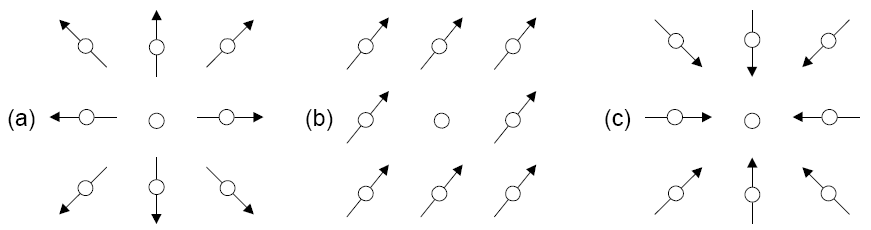
\includegraphics{images/convergence-index.png}
\caption{O índice de convergência é calculado a partir do aspecto das
oito células vizinhas. O exemplo mostra (a) divergência total, (b)
superfície plana e (c) convergência total. Adaptado de (Conrad, 1998).}
\end{figure}

\section{Índice de exposição ao
norte}\label{indice-de-exposicao-ao-norte}

(northerness): descreve o grau de exposição de uma determinada ao ponto
cardeal norte; Northerness: (sinônimo: algum?; inglês -- northerness;
unidade - graus): atributo local que indica a direção da vertente em
relação ao norte. Obtido através da seguinte equação: Northerness =
\textbar{}180 -- aspecto\textbar{}, onde aspecto é o azimute da
declividade expresso em graus no sentido horário a partir do norte,
representando a primeira derivada da superfície de elevação ao longo do
declive, paralelo às curvas de nível. O aspecto possui influência sobre
a insolação, evapotranspiração, e a distribuição e abundância da flora e
da fauna (Wilson \& Gallant, 2000a). Mas como o aspecto constitui uma
medida circular, seus valores não são adequados para comparação direta,
sendo necessária a sua transformação para northerness (Roecker \&
Thompson, 2010). O exemplo apresentado abaixo foi calculado utilizando o
método de Zevenbergen \& Thorne (1987).

\section{Índice de exposição ao norte da área à
montante}\label{indice-de-exposicao-ao-norte-da-area-a-montante}

Catchment aspect

Descreve o grau de exposição médio das células da área à montante (área
de contribuição) de uma determinada célula ao ponto cardeal norte. Está
diretamente relacionado à entrada de energia radiativa, cujos efeitos
são descritos abaixo. A principal diferença é que constitui um atributo
de terreno secundário, indicando qual é o processo predominante que
ocorre na área de contribuição de uma determinada célula. Além disso, o
índice de exposição ao norte da área à montante indica a exposição do
terreno aos ventos dominantes, os quais possuem efeito significati vo
sobre a distribuição do tamanho de partículas em diversas partes do
mundo através da erosão eólica. OBS.: o índice de exposição ao norte é
usado como forma de linearização do atributo aspecto ou orientação, o
qual é um atributo circular e, portanto, inadequado para a construção de
modelos matemáticos.

\section{Índice de potência de
escoamento}\label{indice-de-potencia-de-escoamento}

(stream power index): descreve o potencial de acumulação do fluxo hídrico
e de escoamento superficial. Índice de potência de escoamento: (sinônimo
-- índice de capacidade de trasnporte de sedimento; inglês -- stream
power index, sediment transport capacity index; unidade -- adimensional)
atributo regional desenvolvido por Moore et al. (1988), trata-se de uma
medida do potencial erosivo da enxurrada. Com o aumento da área de
contribuição específica e da declividade, a quantidade de água que chega
das áreas a montante e a velocidade do fluxo da água aumentam, levando
ao consequente aumento da potencial de escoamento e de erosão (Gruber \&
Peckham, 2009). O índice de potência de escoamento (IPE) é obtido
através da seguinte equação:

\[IPE = AC_s \times \tan(\beta)\]

onde \(AC_s\) é a área de contribuição específica (m\textsuperscript{2}
m\textsuperscript{-1}) e \(\beta\) é a declividade (graus). O IPE pode
ser utilizado para identificar os locais onde medidas de conservação do
solo que reduzem os efeitos erosivos do escoamento concentrado podem ser
adotadas (Moore et al., 1991).

\section{Índice de proteção
morfométrica}\label{indice-de-protecao-morfometrica}

(morphometric protection index): descreve como o relevo ``protege''
(fecha-se sobre) uma determinada célula a partir da sua relação
morfométrica com as células vizinhas (de- clividade e orientação).
morphometric protection index (openess): this algorithm analyses the
inmediate surrounding of each cell up to an given distance and evaluates
how the relief protects it → relacionada com a curvatura.

\section{Índice de resolução múltipla de nivelamento de fundo de
vale}\label{indice-de-resolucao-multipla-de-nivelamento-de-fundo-de-vale}

(multiresolution index of valley bottom flatness): descreve o quão plano
é o fundo de um vale; mapping of depositional areas

\section{Índice de resolução múltipla de nivelamento de topo de
morro}\label{indice-de-resolucao-multipla-de-nivelamento-de-topo-de-morro}

(multiresolution index of ridge top flat- ness): descreve o quão flano é o
topo de um morro;

\section{Índice de rugosidade do
terreno}\label{indice-de-rugosidade-do-terreno}

Terrain ruggedness index

Descreve a heterogeneidade (rugosidade) de uma superfície em função do
gradiente da elevação entre células vizinhas. A rugosidade do terreno
impõe restrições ao fluxo de água de uma célula à outra, fazendo-o estar
intimamente relacionado à erosão do solo. Além disso, o índice de
rugosidade do terreno costuma ser usado como indicativo de afloramentos
rochosos e deslizamentos de massa. Nesses locais o solo é pouco
desenvolvido e a proporção das frações mais finas da distribuição do
tamanho de partículas costuma ser pouco significativa.

Índice de rugosidade da superfície: (sinônimo -- algum?; inglês --
terrain eggedness index; unidade -- adimensional): atributo desenvolvido
por Riley et al. (1999) que quantifica a heterogeneidade da superfície.
Está relacionado aos processos de formação do solo, a geomorfologia e a
distribuição da fauna e da flora. O índice é calculado a partir da soma
da mudança de elevação entre uma célula e as suas oito células vizinhas.

\begin{figure}[htbp]
\centering
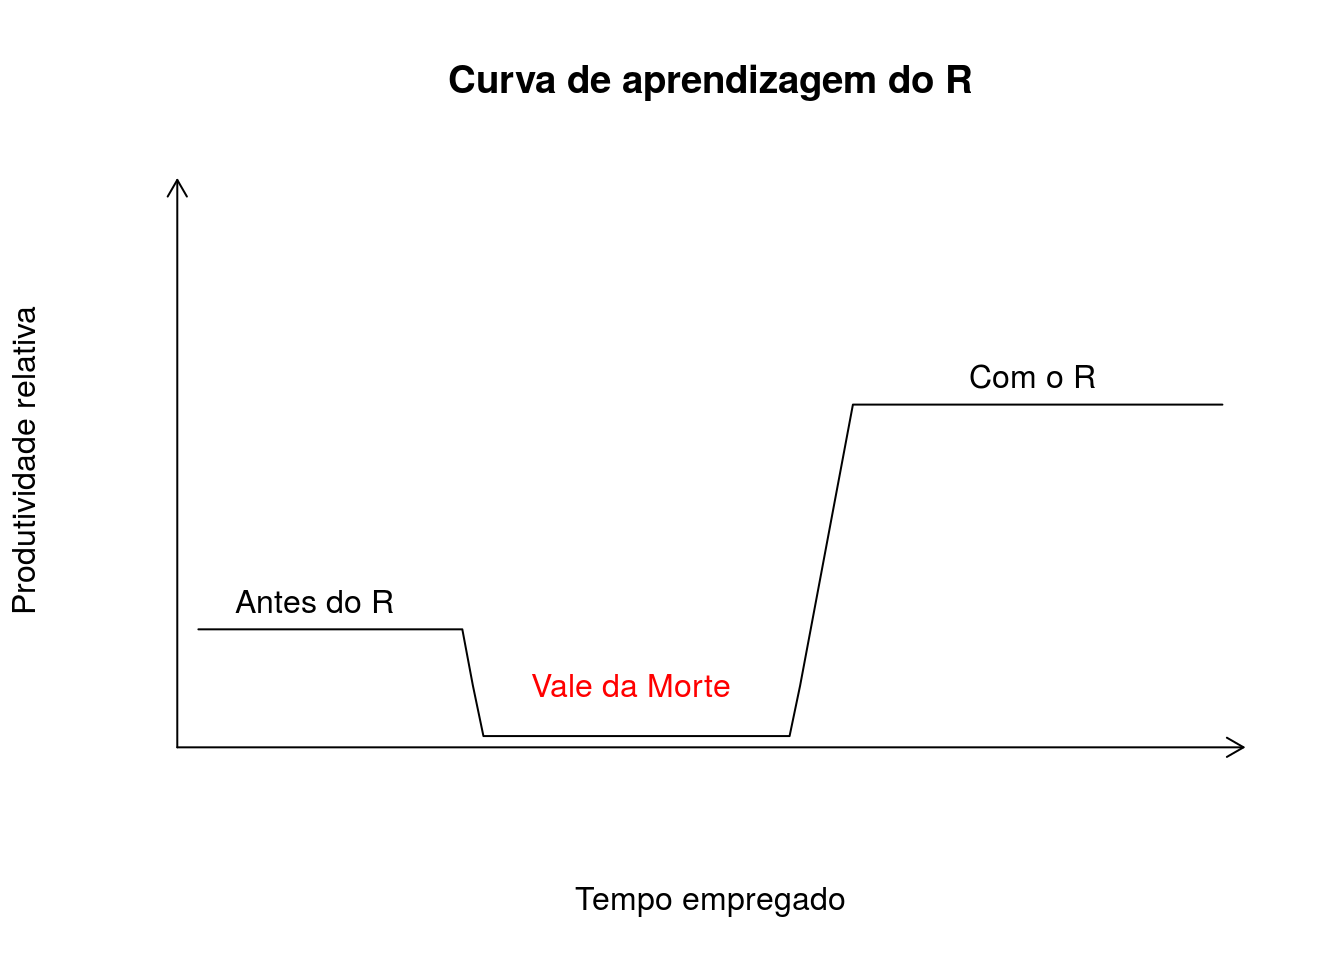
\includegraphics{pedologia-quantitativa_files/figure-latex/unnamed-chunk-8-1.pdf}
\caption{\label{fig:unnamed-chunk-8}Representação de uma janela de 3 por 3
células de uma superfície de elevação para o cálculo do Índice de
Rugosidade da Superfície. Adaptado de Riley et al. (1999).}
\end{figure}

Se cada quadrado na figura acima representa uma célula de uma superfície
de elevação, então o IRS é dado pela seguinte equação:

\[IRS = y \sqrt{\sum (x_{ij} - x_{00})^2}\]

onde \(x_{ij}\) é a elevação de cada célula vizinha a célula (0, 0). Os
valores de IRS variam entre os seguintes limites:

\begin{itemize}
\tightlist
\item
  Plano: 0--80 m
\item
  Aproximadamente plano: 81--116 m
\item
  Levemente rugoso: 117--161 m
\item
  Rugosidade intermediária: 162--239 m
\item
  Moderadamente rugoso: 240--497 m
\item
  Altamente rugoso: 498--958 m
\item
  Extremamente rugoso: ≥ 958 m
\end{itemize}

Cada classe recebe um número inteiro como identificador.

\section{Índice de umidade
topográfica}\label{indice-de-umidade-topograca}

(topographic wetness index): descreve tendência de uma célula acumular
água; Índice de umidade topográfica: (sinônimo -- algum?; inglês --
topographic wetness index; unidade -- adimensional): atributo local
desenvolvido por Beven \& Kirkby (1978) que descreve a tendência de uma
célula acumular água Gruber \& Peckham (2009). Assim, maiores valores de
índice de umidade topográfica (IUT) indicam maior tendência de acumular
água e, portanto, maior conteúdo de água no solo. O IUT é obtido através
da seguinte equação:

\[IUT = \ln \frac{AC_s}{\tan{\beta}}\]

onde \(AC_s\) é a área de contribuição específica (m\textsuperscript{2}
m\textsuperscript{-1}) e \(\beta\) é a declividade (graus). Contudo,
essa equação assume condições estáveis e solos com propriedades
uniformes, ou seja, a transmissividade é constante ao longo da bacia e
igual à unidade (Wilson \& Gallant, 2000a). Como a variação do
componente topográfico é comumente maior do que a variação da
transmissividade do solo (Wood et al., 1990), essa equação pode ser
usada na maioria das superfícies geomórficas.

\section{Insolação potencial}\label{insolacao-potencial}

Potential incoming solar radiation

Descreve a quantidade de energia radiativa que pode atingir uma
superfície em um determinado período de tempo. Essa energia move a
grande maioria dos processos atmosféricos, hidrológicos e biológicos que
ocorrem nas imediações da superfície terrestre. Diferentes entradas de
energia resultam em diferenças nas taxas dos processos biogeoquímicos,
sobretudo porque a disponibilidade de água é diferenciada, afetando
diretamente a taxa de intemperismo. Como consequência, pode haver efeito
sobre a distribuição do tamanho de partículas do solo de acordo com a
entrada de energia radiativa.

Largura do fluxo (flow width): descreve a largura alcançada pelo
escoamento superficial

\section{Posição em relação ao meio da
encosta}\label{posicao-em-relacao-ao-meio-da-encosta}

Mid-slope position

Descreve a posição da célula em relação ao meio da vertente. Geralmente
é utilizado como indicator topoclimático, ou seja, descreve o efeito da
topografia sobre as condições climáticas. O principal efeito descrito é
a mudança da temperatura em direção às partes mais altas (picos) e às
partes mais baixas do terreno (vales) em regiões de relevo bastante
acidentado, onde as temperaturas mais quentes podem vir a ocorrer nas
posições intermediárias da paisagem. Assim sendo, a posição em relação
ao meio da encosta constitui outro atributo de terreno relacionado com a
disponibilidade de energia e, portanto, aos ciclo biogeoquímicos, assim
como a insolação potencial e o índice de exposição ao norte.

Profundidade do vale (valley depth, height below summit): descreve a
distância vertical da célula até o topo da encosta;

\section{Rugosidade vetorial do
terreno}\label{rugosidade-vetorial-do-terreno}

Vector ruggedness index

Descreve a heterogeneidade (rugosidade) de uma superfície em função do
gradiente da elevação entre células vizinhas, assim como o índice de
rugosidade do terreno. A diferença é que o índice de rugosidade vetorial
é menos dependente da declividade e captura a variação da declividade e
do aspecto em uma única medida. Sua relação com a distribuição do
tamanho de partículas é exatamente a mesma apresentada pelo índice de
rugosidade do terreno.

Sinuosidade do escoamento superficial (flow sinuosity): descreve a relação
entre o caminho percorrido pelo escoamento superficial de uma célula até
o exutório e a distância Euclideana entre a célula e o exutório.

\bibliography{packages.bib,book.bib}


\end{document}
